\section{Discussion}
\label{sec:discussion}
This section explores the results stated in the previous section and attempts to find explanations or new connections between topics. Since there are multiple angles to discuss the results from the section has been split up to multiple subsections.

\subsection {System call sets}
\begin{figure}
    \centering
    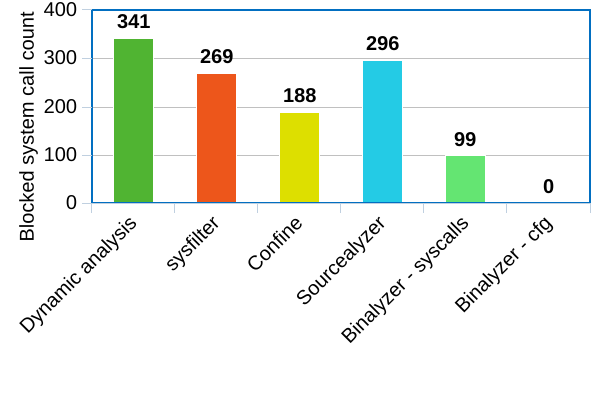
\includegraphics[width=\columnwidth]{./chart_syscalls.png}
    \caption{Blocked system call count for all investigated analysis tools for sqlite.}
    \label{fig:block_count}
\end{figure}
When looking at the results it is evident that the dynamic analysis solution developed for this research blocks the largest amount of system calls, as shown on Figure \ref{fig:block_count}.
However it is important to mention that this result is only as strong as the analysis cases that are exercising the program under test, and therefore it is possible that some execution path is missed.
This leads to underestimating the set of required system calls, and if these system calls were truly blocked it might stop the applications from working under certain conditions that were not explored during testing.
It is difficult to come up with a comprehensive analysis suite, since the behavior depends not only on the inputs to the program but also on the state of the system as a whole.

In comparison static analysis tools block less system calls, and they potentially overestimate the set of required system calls, depending on how much information about the program is available and what techniques are used.
However the Sourcealyzer part of Chestnut achieves a close number of blocked system calls to the dynamic analysis solution, demonstrating that the degree overestimation is minimal in some cases.
On the other end of the spectrum, Binalyzer with \textit{syscalls.py} on dynamically linked binaries blocks significantly less calls than any other solution.

Perhaps another positive note about dynamic analysis is that it is possible for the blocked set of system calls to be learned from actual usage of the program. If only a part of the built-in functionality of a program is used in a given system, it can be safer to block system calls related to the unused functions. This concept is not captured by purely static analysis based tools, which first slightly overapproximate the required set of system calls and then offer no solution to reduce the size of this set.

\subsection {Analysis time}
\begin{figure}
    \centering
    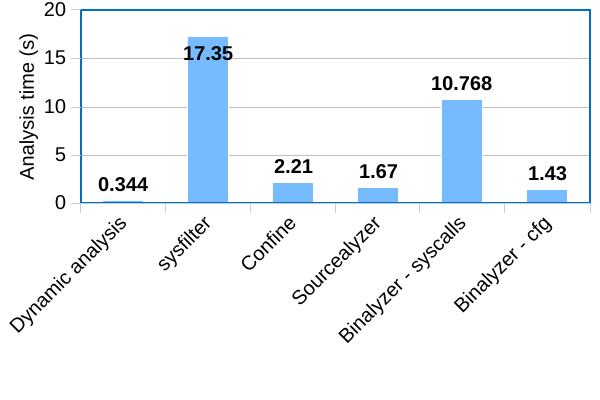
\includegraphics[width=\columnwidth]{./chart_timings.png}
    \caption{Analysis times for all investigated analysis tools for sqlite.}
    \label{fig:timings}
\end{figure}
From the aspect of analysis time it can be seen that the dynamic analysis solution takes the least amount of time, as shown in Figure \ref{fig:timings}, therefore it leaves room for more analysis cases to be added, until the analysis time approaches that of the static analysis tools.

The second fastest solution is confine with 1-2 seconds spent per program on average. This is because confine contains a pre-computed call graph for certain libc versions, and thus skips the steps where most analysis tools spend their time, analyzing what systems calls the libc functions make that are used by the given program. Therefore a promising technique to speed up analysis could be precomputing results for popular libraries and dependencies.

The next fastest solution is perhaps surprisingly the Sourcealyzer part of Chestnut, with 1-4 seconds of analysis time per program. Although this may be unexpected a first, a significant speedup is achieved by utilizing multiple cores. Since the Sourcalyzer is implemented as an LLVM pass it has the same parallelization options as other compiler tasks, and thus allowing 16 concurrent jobs while testing greatly favors solutions which take advantage of multiple cores. In comparison, all of the other solutions relied on single core execution, therefore another opportunity to increase analysis speeds is to utilize multiple cores.

Perhaps the slowest solution is the Binalyzer part of Chestnut, specifically using the \textit{cfg.py} script.
This demonstrates the CFG construction is a time consuming task, and also nicely demonstrates that as program size scales up from \textit{ls} to redis, execution time also increases from 11 seconds to 1 minute. This further highlights the benefit that static analysis solutions aim to find faster, but potentially less accurate ways to find out which functions are called, and which system calls are connected to those functions.

\subsection {Setup \& Usability}
Although the above detailed metrics are of most importance, the adoption of these technologies depends on how easy they are to setup and use. Additionally it is an important aspect to consider when choosing a tool. For example a longer analysis time might be acceptable if the setup and use is much easier compared to the other tools.

The dynamic analysis solution is relatively simple, it is easy to compile and run. The analysis cases are easily expandable, however it is tedious to come up with an analysis suite that adequately covers the program space. Additionally, the risk of mistakenly blocking a system call might outweigh the advantages of the easier setup and use.

In the case of sysfilter the setup is relatively easy and the analysis software worked well on the tested binaries. A potential problem here is the distribution or package versions used, as running the program on ubuntu 16.04 leads to the analysis tool crashing during analysis.

For Confine the setup is similarly easy and the analysis software worked well, and although on the test system there were problems with \textit{sysdig}, luckily other monitoring tool options were also supported.
Here a potential problem is with containers that are not long running, and exit within 60 seconds of starting. The analysis tool is designed for long running containers and attempts to analyze a simple container that exits almost immediately after starting have been unsuccessful.

In the case of chestnut, the setup is pretty cumbersome, as no guide or detailed instructions are available on how to setup a system to work with chestnut.
The setup is more time consuming compared to other tools, due to the large amount of compilation work.
Additionally the implementation is restrictive in the compiler used, its version, and the need for static compilation.
In the end, although the filtered system calls were extracted, the produced binaries crashed early in the loading process and were not able to run.
Although it is possible that the setup has mistakes, it highlights the problem of missing setup and usage instructions.
